\documentclass{article}
\usepackage{tikz}
% \usepackage{xfp}
% \usetikzlibrary{math}


\ExplSyntaxOn
\newcommand\calcu[1]{\fp_eval:n {#1}}
\ExplSyntaxOff

\begin{document}
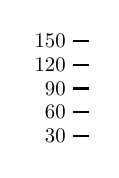
\begin{tikzpicture}
  \foreach \y in {.3, .6, .9, 1.2, 1.5}{
    % \tikzmath{\yy=100*\y;}
    \draw[thick] (2, \y) node [left, scale=.75]
      {\fpeval{\y*100}} --++ (.2, 0);
      % {\calcu{\y*100}} --++ (.2, 0);
      % {\yy} --++ (.2, 0);
  }
\end{tikzpicture}

\end{document}